\chapter{Realisierung}\label{ch:realisierung_der_anwendung}
In den nachfolgenden Abschnitten werden alle für die Implementierung wichtigen technischen Aspekte und deren Umsetzung erläutert. Es wird einen Einblick in die Arbeitsweise mit dem AR-Framework Vuforia im Zusammenspiel mit dem Rendern von 3D Objekten gegeben. Des Weiteren wird die interne Datenhaltung, sowie die Umsetzung einzelnen Szenen in Unity beschrieben.

\section{Einbindung der Mustererkennung}\label{einbindung_mustererkennung}
In Abschnitt \ref{mustererkennung_vuforia} wurde bereits näher die internen Funktionsweise des Augmented Reality Frameworks \textquote{Vuforia} erklärt. 
Um dessen vollen Umfang in der Unity-Projektumgebung nutzen zu können, musste das entsprechende Vuforia Software Development Kit eingebunden werden.
Es beinhaltet im Wesentlichen alle Grundbausteine für die Entwicklung einer Augmented Reality App und stellt diese in Form von Unity GameObjects (vgl. Abschnitt \ref{aufbau_unity_app}) bereit. 
Dadurch sind sie genau wie herkömmliche GameObjects nutzbar und können einfach in ein bestehendes Unity-Projekt integriert werden, um dieses zu erweitern.

Ein Beispiel für einen solchen Baustein ist die AR Camera. 
Sie beinhaltet Logik, um die Hauptkamera des ausführenden Gerätes anzusteuern. 
Die Szene in der die Kamera platziert wurde, wird nun in das Kamerabild der realen Welt projiziert.
Dieser Baustein ist essentiell für die Erstellung einer Augmented Reality App. 

Auf einen weiteren essentiellen Baustein aus der Vuforia SDK wird in den nachfolgenden Unterabschnitten \ref{image_targets} und \ref{integration_image_targets} eingegangen. 

\subsection{Image Targets}\label{image_targets}
Da wir uns in der Anwendung für die markerbasierte Variante der Augmented Reality entschieden haben, benötigen wir hierzu die passenden Marker. 
Wie bereits in Abschnitt \ref{mustererkennung_vuforia} beschrieben, bietet Vuforia hier die Möglichkeit, eigene Image Targets zu verwenden. 
Da diese innerhalb der Anwendung möglichst gut erkannt werden sollen, müssen bei der Wahl der Bilder einige Qualitätskriterien beachtet werden.

Eines dieser Kriterien sind die Ecken und Kanten im Bild, welche durch die Featureextraktion beim Hochladen des Bildes berücksichtigt werden. 
Jede scharfe Ecke und Kante wird als Feature abgespeichert und dient später bei der Bilderkennung innerhalb der Anwendung als Vergleichsmerkmal. 
Je mehr dieser markanten Punkte im Bild vorhanden sind, desto leichter fällt es der Vuforia Engine das Image Target im Kamerabild der AR-Anwendung zu identifizieren.

Um sicherzugehen, dass aus dem gewählten Image Target viele Features extrahiert werden können, sollte das Bild hohe lokale Kontraste besitzen. Das heißt, es sollte ausreichen viele Stellen geben, an denen sehr helle Pixel neben sehr dunklen liegen. 
Hiermit ergeben sich ausgeprägte Farbunterschiede und somit schärfere Ecken und Kanten, welche als potentielle Features in Frage kommen.

\begin{figure} [h]
\centering
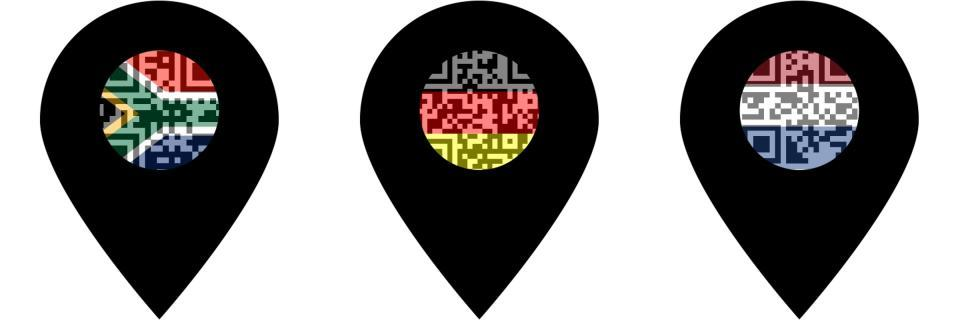
\includegraphics[width=12cm]{Image_Targets.jpg}
\caption{Beispiele der verwendeten Image Targets}
\label{fig:image_targets}
\end{figure}

In Abbildung \ref{fig:image_targets} sind die finalen Image Targets der beschriebenen Anwendung zu sehen.
Die Grundform der Targets stellt die heutzutage sehr häufig genutzte Form des Standortsymbols dar.
Wir wählten die Form um die Erdkundethematik der Anwendung zu unterstreichen.
Diese werden in der Praxis auf einem Globus platziert und jedes Target repräsentiert ein Land.
Um die Verbindung zu dem jeweiligem Land erkenntlich zu machen, ist Flagge des Landes in das Standortsymbol integriert. 
Somit ist jedes Image Target einzigartig und lässt sich von den anderen unterscheiden. 
Der Nutzer der Anwendung kann jetzt erkennen, welches Image Target zu welchem Land gehört und kann sich gleichzeitig die Flaggen der Länder einprägen. 

Nun sind zwar alle Targets einzigartig und können in manchen Fällen sehr gut unterschieden werden, jedoch ist das noch nicht ausreichend um bei der Targeterkennung befriedigende Ergebnisse zu erhalten. 
Bei der Merkmalsextraktion werden die Bilder in Graustufen umgewandelt und verlieren somit jegliche Farbinformationen. Dies kann beispielsweise bei den Flaggen von Deutschland und den Niederlanden zu Schwierigkeiten in der Unterscheidung führen, da sie aus den exakt gleichen Formen bestehen. 
Die Ecken- und Kantenmerkmale wären damit sehr ähnlich. 
Um dieses Problem zu lösen, hinterlegten wir jede Flagge mit einem individuellem QR-Code. 
Dieser ist leicht transparent, bringt aber dennoch mehr Kontrast in das Bild. 
Somit können selbst aus den einfach geformten Flaggen genügend eindeutige Merkmale erzeugt werden.

Diese Art der Image Targets resultiert in der Vuforia Engine in einer Fünf-Sterne Erkennungsrate.

\subsection{Integration der Image Targets}\label{integration_image_targets}
Nachdem nun alle fertigen Image Targets über das in Abschnitt \ref{mustererkennung_vuforia} beschriebene Target Management System geladen wurden, müssen diese in die Anwendungsumgebung integriert werden.
Hierzu wird aus der Weboberfläche eine Datenbank erzeugt, die alle Targets enthält. 
Anschließend wird sie als \textquote{.unitypackage}-Datei heruntergeladen und kann in das bestehende Unityprojekt importiert werden.

Um nun die einzelnen Image Targets innerhalb der Anwendung nutzbar zu machen, wurde zunächst eine dedizierte Szene erstellt. 
In dieser Szene befindet sich zuerst einmal die AR Camera, welche in Abschnitt \ref{einbindung_mustererkennung} beschrieben ist. 
Des Weiteren wird für jedes vorhandene Land das passende Target benötigt.
Ein Image Target wird in Form eines GameObjects in die Szene geladen.
Es ist ein spezieller Typ von GameObject, welcher von der Vuforia-SDK mitgeliefert wird und bereits vordefinierte Logik in Form von Komponenten enthält.
Ein Beispiel hierfür ist die Scriptkomponente \textquote{Image Target Behaviour}, welche die Kommunikation mit der Image Target Datenbank regelt. 
Sie bietet die Möglichkeit, zwischen allen importierten Datenbanken und den darin enthaltenen Image Targets zu wählen.
Wählt man jetzt beim ersten GameObject das Target des Landes Indien, so erscheint an der Stelle des vorher leeren Objekts, das erstellte Image Target für genau dieses Land.
Dieser Vorgang muss nun für alle restlichen Länder wiederholen, damit alle in der Szene enthalten sind.

Wenn nun die fertige Szene gestartet wird, öffnet sich zunächst die Kamera des ausführenden Geräts.
Im Hintergrund wird das Kamerabild ständig untersucht und geprüft, ob sich eines der in der Szene liegenden Image Targets im Sichtfeld befindet. Im Falle einer Bilderkennung können unterschiedliche Aktionen ausgeführt werden, welche in Abschnitt \ref{einbindung_3D_objekte} genauer beschrieben werden.

\section{Verwendung von 3D Objekten}\label{verwendung_3d_objekte}
Die in der Anwendung verwendeten 3D Objekte liegen im \textquote{object}-Format vor, welches durch die Dateiendung \textquote{.obj} gekennzeichnet ist. 
Dem Dateiformat liegt das polygonale Modell zugrunde, das 3D Objekte als Zusammensetzung von Polygonen, die wiederum aus durch Kanten verbundenen Koordinaten bestehen, definiert. 
Die geläufigsten so entstehenden Polygonnetze sind Dreiecksnetze und Vierecksnetze.

In einer  \textquote{.obj}-Datei sind somit die Koordinaten von Punkten im dreidimensionalen Raum definiert, welche über Kantendefinitionen zu Flächen verbunden werden. 
Um 3D Objekte realistisch erscheinen zu lassen, findet der Prozess des sogenannten \textquote{Texture Mappings} statt, in welchem eine Textur im Bildformat über ein 3D Objekt gelegt wird. 
Auf Codebasis wird dies realisiert, indem in der \textquote{.obj}-Datei zweidimensionale Texturkoordinaten für eine vorhandene Textur definiert und bestimmten Punktkoordinaten des Objekts zugewiesen werden.

Primitive 3D Objekte, die aus wenigen Polygonen bestehen, können somit leicht selbst erstellt werden, während die Erstellung von komplexeren Objekten und zugehörigen Texturen mehr Zeitaufwand erfordert. 
Da dieser Zeitaufwand nicht in den zeitlichen Rahmen dieses IT Projektes gepasst hat, haben wir uns dafür entschieden, kostenlose 3D Objekte mit zugehörigen Texturen von verschiedenen Anbietern aus dem Internet zu verwenden, welche im folgenden aufgelistet sind.

\begin{itemize}
\item https://www.turbosquid.com/
\item https://www.cgtrader.com/
\item https://free3d.com/
\end{itemize}

Wie bereits in Abschnitt \ref{projektziel} erwähnt, sollen die in der App enthaltenen Länder durch passende 3D Objekte repräsentiert werden, welche auf das erkannte Image Target eines Landes gerendert werden. 
Die folgende Auflistung zeigt die gewählten 3D Objekte für ihre zugehörigen Länder, gegliedert in Kontinente. Diese sind bildlich auch im Anhang dargestellt.

\textbf{3D Objekte für Afrika:}
\begin{itemize}
\item Kongo: Affe
\item Südafrika: Elefant
\item Ägypten: Pyramide
\end{itemize}

\textbf{3D Objekte für Europa:}
\begin{itemize}
\item Deutschland: Brandenburger Tor	
\item Frankreich: Eiffelturm
\item Niederlande: Windmühle
\end{itemize}

\textbf{3D Objekte für Nordamerika:}
\begin{itemize}
\item Kanada: Hirsch
\item USA: Empire State Building
\item Mexico: Maya Tempel
\end{itemize}

\textbf{3D Objekte für Südamerika:}
\begin{itemize}
\item Brasilien: Palmenwald
\item Argentinien: Pinguine
\item Peru: Machu Picchu
\end{itemize}

\textbf{3D Objekte für Asien:}
\begin{itemize}
\item Indien: Taj Mahal
\item Malaysia: Petrona Towers
\item Japan: Tempel
\end{itemize}

Die Einbindung dieser 3D Objekte und die dazu nötige Vorverarbeitung dieser werden in den folgenden Abschnitten beschrieben.
\subsection{Vorverarbeitung}
Die Vorverarbeitung der 3D Objekte wurde mit dem kostenlosen Grafikprogramm \textquote{Blender} realisiert, welches einen großen Funktionsumfang für die Bearbeitung und Erstellung von 3D Körpern bietet. 

Die vorherige Bearbeitung der 3D Objekte war hauptsächlich aus zwei Gründen nötig. 
Zum Einen erleichterte sie die Einbindung der Objekte, da die aus unterschiedlichen Quellen stammenden 3D Objekte meist sehr groß skaliert und rotiert waren.
Durch einfache Transformationsoperationen konnten diese Objekte somit auf eine einheitliche Größe und Ausrichtung normalisiert werden, wodurch die aufwendigere Bearbeitung in Unity nicht mehr nötig war.

Ein weiterer Anwendungsfall für die nötige Vorverarbeitung der 3D Objekte in Blender war die nötige Reduktion der Polygonzahl der Objekte. 
Die aus dem Internet stammenden Körper wiesen eine sehr hohe Polygonzahl auf und waren dadurch sehr hoch aufgelöst, was zu einer größeren Dateigröße und somit einer Belastung des Anwendungsspeichers führen würde. 
Eine solch hohe Auflösung war in unserem Anwendungsfall nicht nötig, da die 3D Objekte auf dem Globus sehr klein skaliert angezeigt werden und die gegebenen Genauigkeiten somit nicht auffallen würden. 
Um Speicherplatz innerhalb der App zu sparen wurde die Polygonzahl und damit die Dateigröße der 3D Objekte mithilfe von Blender um das zehnfache verringert, bevor diese in der App eingebunden wurden.

Die Veränderung der Polygonzahl wird durch Grafiken \ref{fig:elefant_viele_polygone} und \ref{fig:elefant_wenig_polygone} dargestellt.

\begin{figure}[!htb]
\minipage{0.48\textwidth}
  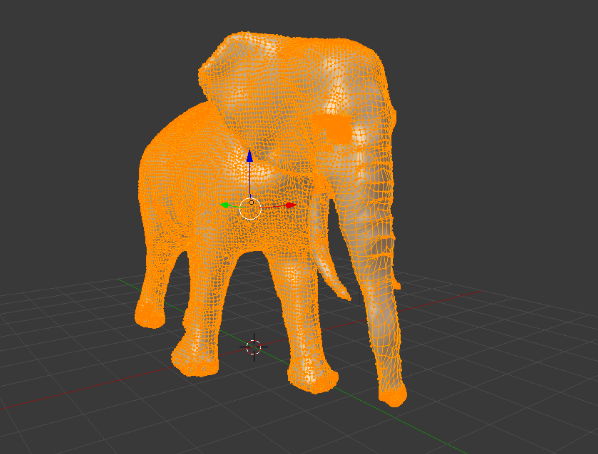
\includegraphics[width=\linewidth]{elefant_viele_polygone.png}
  \caption{Polygonnetz vor Bearbeitung}\label{fig:elefant_viele_polygone}
\endminipage\hfill
\minipage{0.48\textwidth}
  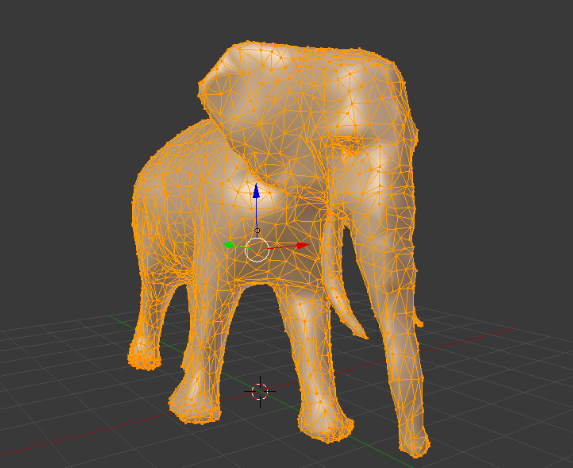
\includegraphics[width=\linewidth]{elefant_wenig_polygone.png}
  \caption{Polygonnetz nach Bearbeitung}\label{fig:elefant_wenig_polygone}
\endminipage\hfill
\end{figure}

Aus Grafik \ref{fig:elefant_wenig_polygone} geht hervor, dass sich die Gestalt des 3D Objektes trotz verringerter Polygonzahl kaum verändert und der Prozess der Polygonreduktion somit zu einem nicht merklichen Genauigkeitsverlust führt.
\subsection{Einbindung der 3D Objekte in Unity}\label{einbindung_3D_objekte}
Der Zugriff auf die ausgewählten 3D Objekte innerhalb des Unity-Entwicklungsoberfläche, sowie der Applikation wird ermöglicht, indem die Objekte im Projektpfad als Ressourcen abgelegt werden, welche beim Bauen der Applikation auf das Endgerät mit übertragen werden. 

Wie in Abschnitt \ref{projektziel} beschrieben, soll ein 3D Objekt nur bei der Erkennung des ihm zugeordneten Landes angezeigt werden.
Um dies zu realisieren, werden die 3D Objekte in der Entwicklungsoberfläche als Kind-Objekte der in Abschnitt \ref{integration_image_targets} beschriebenen Image-Targets angelegt.
Das Verhalten dieser Vuforia-Elemente wird durch das \textquote{DefaultTrackableEvent-Handler}-Skript bestimmt, welches den Elementen standardmäßig beigefügt ist. 
Bei der Feuerung des \textquote{OnTrackableFound}-Events, das heißt der Erkennung eines Image-Targets, werden die diesem untergeordneten, renderbaren Kindelemente mithilfe der von Unity bereitgestellten \textquote{Renderer}-Klasse automatisch gerendert.

Das beschriebene \textquote{DefaultTrackable-EventHandler}-Skript kann nach Belieben bearbeitet werden, um ein besonderes, durch den Benutzer gewünschtes Verhalten hervorzurufen.
In unserem Fall wurde das \textquote{OnTrackable-Found}-Event so erweitert, dass zusätzlich zu dem 3D Objekt noch zwei Buttons angezeigt werden, mit welchen der User interagieren kann.

\section{Verwaltung der Daten}
Im Abschnitt \ref{datenhaltung und -bereitstellung} wurde bereits das geplante Vorgehen für die Erstellung und Verwaltung einer Datenbank mit \textquote{SQLite} erläutert. Der folgende Absatz beschreibt nun das resultierende Datenbankmodell, sowie die Interaktion der Applikation mit den gespeicherten Informationen.
\subsection{Datenbankentwurf}\label{datenbankentwurf}
Aus der Planung haben sich insgesamt fünf Tabellen entwickelt. Die Tabellen \textquote{Information}, \textquote{Question} und \textquote{Answer} dienen hauptsächlich der Speicherung von austauschbaren Inhalten für den Informations- und Lernteil von TraWo. Hier liegen die Informationen, Fragen und Antworten, auf die der Spieler bei der Nutzung der App trifft. Die Tabellen \textquote{Country} und \textquote{Continent} sind eher als Zuweisungstabellen zu betrachten und spielen für die Codierung der Spiels eine große Rolle.

\begin{figure} [h]
\centering
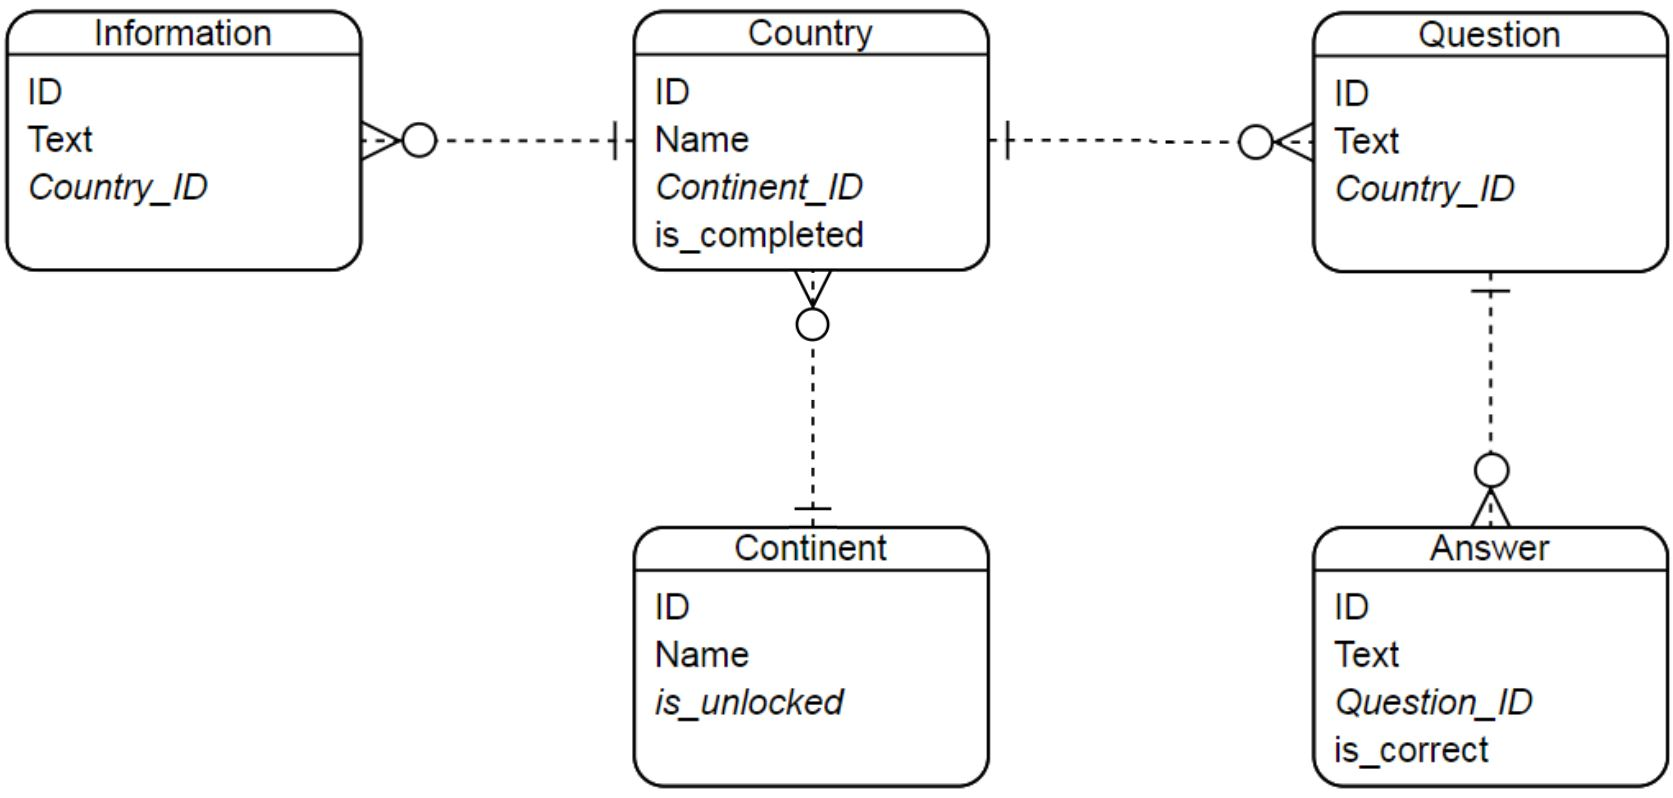
\includegraphics[width=12cm]{Datenbankentwurf.jpg}
\caption{Datenbankentwurf}
\label{fig:db_model}
\end{figure}

Die Grafik \ref{fig:db_model} stellt das Datenbankmodell in der Martin-Notation dar. Die, auch Krähenfußnotation genannte, Darstellung zu \textquote{Entity-Relationship}-Modellen eignet sich, neben Alternativen wie der Chen-Notation, um eine visuelle Repräsentation von Datenbankentwürfen darzustellen. 

Hierbei sollen die semantischen Zusammenhänge zwischen einzelnen Tabellen in Form von Entitäten aufgezeigt werden, die als Rechtecke abgebildet sind. Neben dem Namen des Entitätstypen enthalten sie noch Attribute, welche die Spaltennamen darstellen. Fremdschlüssel sind als Verweis auf andere Tabellen in Form von referenzierten IDs ebenfalls enthalten. Die Beziehungen der Entitäten stellen die Verbindungslinien dar. Diese geben gleichzeitig - über Symbole an den Enden - Aufschluss über die Kardinalität der Entität in der gegebenen Relation. Ein perpendikular zur Verbindungslinie verlaufender Strich steht für \textquote{eins}, der namensgebende Krähenfuß steht für \textquote{mehrere}.

Die im Diagramm gezeigten Beziehungen Beziehungen lassen sich nun wie folgt lesen:
\begin{itemize}
\item Ein Land enthält mehrere Informationen
\item Ein Land enthält mehrere Fragen
\item Ein Kontinent enthält mehrere Länder
\item Eine Frage enthält mehrere Antworten
\end{itemize}

Die Attribute bestehen pro Eintrag zunächst immer aus einer eindeutigen ID. Tabellen mit apprelevanten Inhalten besitzen einen Text, in dem der zugehörige Content gespeichert ist. Zuweisungstabellen besitzen einen Namen. Steht die Tabelle in einer 1:n-Beziehung, so hat die n-seitige Tabelle eine Referenz auf die konkrete, ihr zugehörige Instanz. Beispielsweise hat eine Antwort immer eine passende \texquote{Question\_ID}, damit sie der passenden Frage zugeordnet werden kann. Zuletzt besitzen drei Tabellen einen boolschen-Wert, der wahr oder falsch sein kann. Für die Antworten lässt sich damit bestimmen, ob eine im Quiz angezeigte Antwort richtig oder falsch ist. Für die Länder und Kontinente wird der Wert als Zustandsindikator verwendet. Somit könnte man kennzeichnen, ob für ein Land alle Quizze gelöst wurden, beziehungsweise ob ein Kontinent freigeschaltet und somit spielbar ist.

Das Prinzip ähnelt einem UML-Diagramm für Softwarearchitekturen aus der Softwareentwicklung. Zum einen kann das die Lesbarkeit für alle beteiligten Entwickler erhöhen, selbst wenn sie ansonsten keinen Bezug zu der Datenbankentwicklung hätten, zum anderen kann es sich auch als ein geeigneter Bauplan für die grundlegende Klassenstruktur eines Projektes eignen. Da wir unseren Datenbankentwurf fertig gestellt hatten, bevor wir mit der Ausimplementierung des Codes angefangen haben, ist uns dieser \texquote{Model-First Approach} sehr entgegengekommen.

Im nachfolgenden Abschnitt wird näher auf die technische Umsetzung der Datenbank und deren Einbindung in Unity eingegangen.

\subsection{Zugriff auf Datenbankinhalte}\label{zugriff_datenbank}
Unity ist durch Nutzung der \textquote{Mono.Data.SQLite.dll} in der Lage, SQlite-Befehle auszuführen. Dadurch lassen sich Methoden schreiben, die bei Bedarf mit einer Datenbank interagieren.

Jede dieser Methoden braucht dabei eine Datenbankverbindung und einen ausführbaren SQLite-Befehl. Da sich die Verbindung immer auf die selbe Datenbank bezieht, ist sie als ein konstanter String mit einem relativen Systempfad festgeschrieben. Jeder Aufruf der Datenbank muss diese Verbindung öffnen, und nach Ende des Prozesses wieder schließen. Durch den relativen Pfad wird sichergestellt, dass die Kommunikation mit der Datenbank spezifisch für jedes individuelle Gerät ist. Der Befehl ist dagegen einzigartig für jede Funktion, und erfüllt einen bestimmen Zweck.

Die meisten Methoden sind Lesefunktionen, und sollen somit Inhalte aus der Datenbank auslesen, damit die Anwendung diese verarbeiten kann. Beispielsweise sollen beim Start eines Quiz die möglichen Antworten geladen werden. Die aufgerufene Methode führt nun ein entsprechendes Skript aus und speichert das von der Datenbank kommende Ergebnis in einem \textquote{SqliteDataReader}-Objekt ab. Durch das Iterieren über das Objekt können die Daten konvertiert und weiterverarbeitet werden. Nach diesem Prinzip läuft jeder Datenbankzugriff ab.

Basierend auf dem Datenbankmodell wurden entsprechende Entitäten im Unity-Skript angelegt. Dadurch hat jede Tabelle eine äquivalente C\#-Klasse mit allen dazugehörigen Attributen und Referenzen, die die Datenbankstruktur als Klassenstruktur widerspiegeln. Die beim Auslesen gewonnenen Daten können somit als Objekte weitergereicht und verarbeitet werden. 

Da es sich im gegebenen Modell um eine relativ einfache Struktur handelt, wurde auf die Nutzung von Frameworks wie \textquote{Entity-Framework} verzichtet. Mit der Hilfe von solchen Frameworks, könnte man automatisiert nach dem \textit{Model-First} beziehungsweise \textit{Code-First Approach} passende C\#-Klassen, respektive eine passende Datenbankstruktur erzeugen lassen. Die manuelle Herangehensweise ist allerdings ressourcensparender und gestaltet sich bei kleineren Projekten in der Regel einfacher und übersichtlicher.

Neben den Lesemethoden, wird beim Start von TraWo einmalig ein SQL-Skript zum Erzeugen und Befüllen der eigentlichen Datenbank mit festgeschriebenem Inhalt nach dem obigen Modell ausgeführt. Die Datenbank wird dann lokal auf dem Anwendungsgerät in einer .db-Datei gespeichert und ist zugriffsbereit. 

\section{Realisierung der Anwendung in Unity}
Im Abschnitt \ref{aufbau_unity_app} des Berichts, wurde bereits der generelle Aufbau einer Unity-Anwendung erläutert.
Wie unsere Anwendung nun aufgegliedert ist wird im nachfolgenden Teil behandelt.

Insgesamt besteht die Applikation aus acht Szenen, welche in Abschnitt \ref{prototyp} in Form eines Flowcharts vorgestellt wurden. Angefangen mit der Menüszene, von der aus man entweder in die Onboarding-Szene für das Tutorial, den Spiel- oder den Informationsteil gelangt. 
Der Spiel- und der Informationsteil setzen sich wiederum aus eigenen Szenen zusammen, zu welchen in den nächsten beiden Abschnitten mehr Informationen folgen. 
Die Abbildung \ref{fig:scenegraph} gibt einen gesamten Überblick über die vorhandenen Szenen und deren Übergänge.

\begin{figure} [h]
\centering
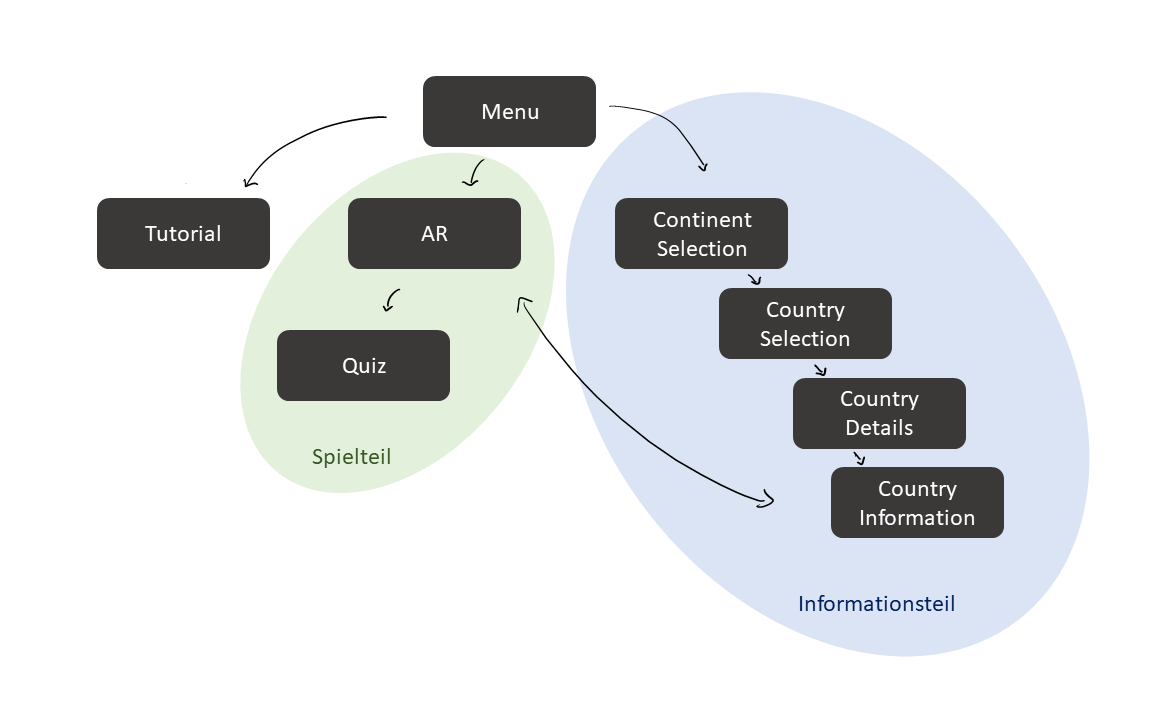
\includegraphics[width=14cm]{Szenenuebersicht.PNG}
\caption{Szenengraph der gesamten Anwendung}
\label{fig:scenegraph}
\end{figure}

Jede Szene besteht aus verschiedenen UI-Elementen, wie beispielsweise Buttons und Textflächen. Je nachdem ob diese mit dynamischer Interaktivität versehen sind, besitzen sie ihr eigenes C\#-Script, welches sich um individuelle Anpassungen kümmert.

\subsection{Informationsbereich}
Der Informationsteil besteht aus vier Einzelszenen. 
In den ersten beiden wählt der Nutzer einen Kontinent und daraufhin ein Land, über das er etwas erfahren möchte.
Anschließend folgt eine Zwischenszene, welche als Vorschau für das gewählte Land dient und danach startet die eigentliche Informationsszene. 

Um den ganzen Bereich dynamisch zu halten, befinden sich in den Szenen nur Dummyobjekte, welche noch nicht mit Texten befüllt sind. Das heißt, dass beispielsweise die Kontinentauswahl vorerst nur leere Buttons und die Informationsszene leere Informationsfelder enthält.
Durch die in Abschnitt \ref{zugriff_datenbank} beschriebene Datenbankschnittstelle, werden diese nun beim Laden der Szene mit Inhalten befüllt. 
In diesem Zuge werden die leeren Auswahlbuttons in der Kontinent- und der Länderszene, dem Styleguide entsprechend unterschiedlich eingefärbt. Und die leeren Informationsfelder werden mit hilfreichen Fakten beschrieben.
Dies wird im Folgenden am Beispiel der Informationsszene verdeutlicht.

Zunächst werfen wir einen Blick auf die vorangehende Szene, in welcher ein Land gewählt wird. 
Beim Tippen auf eines der wählbaren Länder wird das \textquote{Behaviour-Script} dieser Szene aufgerufen, in dem sich ein \textquote{onClick-Event} befindet. 
In diesem wird der Inhalt des angeklickten Objekts, also der Name des jeweiligen Landes, ausgelesen und zwischengespeichert. 
Nun kann er als Parameter an die Datenbankfunktion weitergereicht werden, welche für das Laden der Informationen eines Landes zuständig ist. 
Die daraus resultierenden Daten stehen nun in der darauffolgenden Informationsszene in Form einer Liste zur Verfügung.
Beim Laden der Szene wird deren Behaviour-Script geladen und die darin enthaltene \textquote{Start}-Methode ausgeführt. Diese dient zur Initialisierung der Szene und verarbeitet die vorher erlangten Daten.
Es wird mithilfe einer Schleife über die zwischengespeicherten Informationstexte iteriert, und für jeden Textblock in der Szene wird das jeweilige Textattribut ersetzt.
Die GameObjects der Textblöcke für die einzelnen Informationen müssen hierfür vorher im Script referenziert werden, damit darauf zugegriffen werden kann.

\begin{figure} [h]
\centering
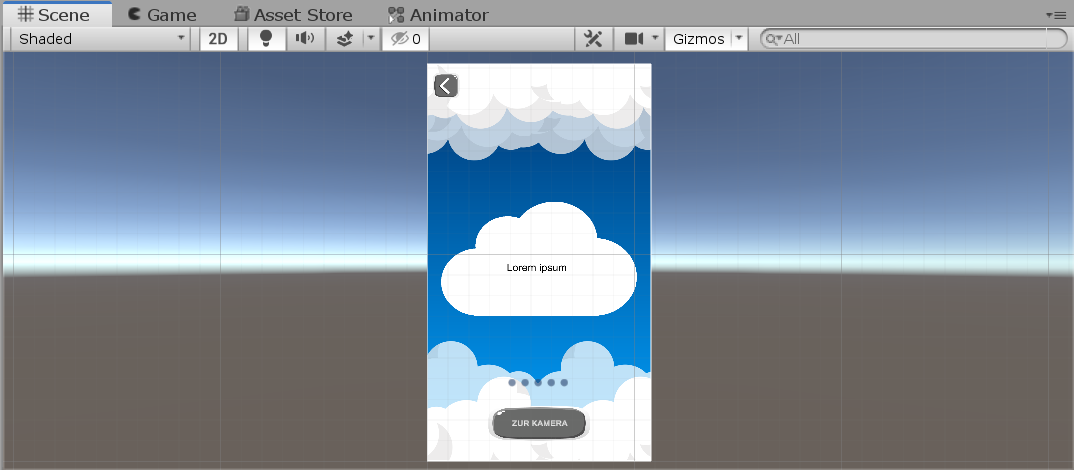
\includegraphics[width=14cm]{Informationsszene.PNG}
\caption{Initialer Status der Informationsszene}
\label{fig:infoscene}
\end{figure}
Die genannten Informationstexte sind in einzelne Elemente aufgeteilt, welche sich innerhalb eines horizontal scrollbaren Containers befinden. 
Es ist immer nur ein Informationselement sichtbar und mithilfe einer Wischgeste kann der Nutzer zur nächsten Information wechseln.
Die in Abbildung \ref{fig:infoscene} erkennbare kleine Anzeige unterhalb des Informationsfeldes zeigt an, welches der fünf Informationsfelder gerade gezeigt wird.
Diese Anzeige wird auch \textquote{Pagination} genannt, da sich die einzelnen Elemente wie scrollbare Seiten verhalten.
Für die Scrollbox und die Pagination musste ein externes Unity Packet installiert und importiert werden, welches beide Funktionen in Form neuer GameObjects hinzufügt.
Die Szenenhierarchie der Informationsszene besteht nun aus der Kamera, einem Szenenscript und einem UI-Container. 
Innerhalb des Containers befinden sich die beiden eben genannten Komponenten, sowie ein Button, um in die AR-Szene zu gelangen.

\subsection{Quizbereich}
Ein ähnliches Grundprinzip wurde bei der Umsetzung der Quizszene verfolgt.
Wie in Abbildung \ref{fig:quizscene} zu sehen, wurde die Benutzeroberfläche ebenfalls mit GameObjects vormodelliert, sodass deren Textinhalte aus Platzhalterwerten bestehen.

\begin{figure} [h]
\centering
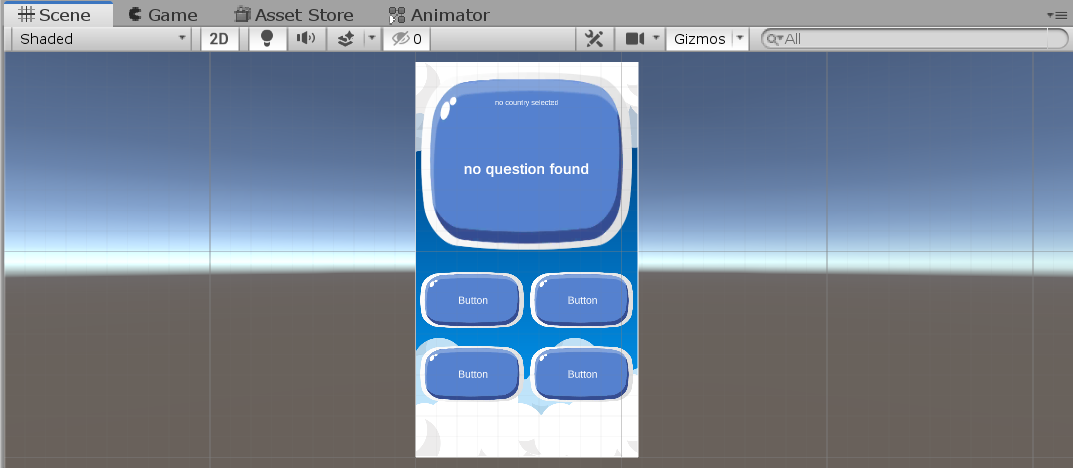
\includegraphics[width=14cm]{quiz_scene.PNG}
\caption{Initialer Status der Quizszene}
\label{fig:quizscene}
\end{figure}

Beim initialen Laden der Szene benötigen wir zuerst die Frage- und Antwortdaten des jeweiligen Landes aus der Datenbank.
Dafür werden erneut Methoden aus der Datenbankschnittstelle, mit dem Übergabeparameter des angeklickten Landes aufgerufen. 
Zuerst laden wir alle Fragen zu dem Land und daraufhin alle Antwortmöglichkeiten zu jeder Frage. 
Die Antwortmöglichkeiten werden an das generierte Frageobjekt angehängt, wodurch eine Liste aus vollständig zusammengesetzten Frageentitäten entsteht.
Diese Liste wird nun innerhalb der Quizszene abgespeichert und kann jetzt, wie im vorher beschriebenen Informationsteil, zum Befüllen der Szene genutzt werden.

Hierfür wird ein C\#-Script benötigt, welches das Verhalten der gesamten Quizszene kontrolliert.
Dieses liegt als eigenes GameObject innerhalb der Szene vor und hält Referenzen auf die in der Szene befindlichen GameObjects.
Es werden die Folgenden benötigt: Der Fragetext, der Text des aktuellen Landes und die vier Buttons der Auswahlmöglichkeiten.
Diese sind alle Objekte die zum Laden eines Quiz nötig sind.

Nun wird Logik benötigt, die über die vorhandenen Fragen iteriert und für jedes Frageobjekt die UI-Texte neu befüllt. Das geschieht innerhalb einer Methode im Script, welche für jede Frage erneut aufgerufen wird. 
Mittels einer Zählervariable weiß sie, welche Frage gerade aktiv ist und befüllt die Szenenoberfläche mit deren Daten.
Hierfür sind die referenzierten GameObjects notwendig, mithilfe derer die Platzhaltertexte überschrieben werden können. 

Damit sich die Reihenfolge der Fragen und die der Antwortmöglichkeiten nicht bei jedem Quizdurchlauf wiederholt, werden sie vorher gemischt. 
Nun müssen wir den Buttons noch \textquote{onClick}-Funktionalität geben. 
Ist eine Antwortmöglichkeit mit dem Flag für \textquote{isCorrectAnswer} versehen, zählt ihr \textquote{onClickListener} einen weiteren Zähler hoch, welcher die korrekten Beantwortungen zählt und ruft anschließend die Initialisierung der nächsten Frage auf. 
Falls nicht, bleibt dieser Zähler gleich und es wird ebenfalls die nächste Frage geladen.

Nach Beantwortung aller Fragen, sollte die erstgenannte Zählervariable der Anzahl an Fragen entsprechen.
Dies dient als Abbruchbedingung des rekursiven Methodenaufrufs zum Laden einer Frage.
Nun wird ausgewertet ob der Nutzer alles richtig beantwortet hat und dementsprechend ein positiver oder ein negativer Feedback-Bildschirm angezeigt.
Dieser informiert darüber ob das Quiz bestanden wurde, zeigt jedoch nicht explizit bei welchen Fragen es nicht geklappt hat.
Von hieraus gelangt man nun durch einen Button wieder zurück zur Kameraansicht der AR-Szene.